\documentclass[a4paper, 11pt]{article}
\usepackage[utf8]{inputenc}
\usepackage{amsmath}
\usepackage{amssymb}
\usepackage{listings}
\usepackage{tabularx}
	\newcolumntype{R}{>{\raggedleft\arraybackslash}X}%
	\newcolumntype{E}{>{\raggedleft\arraybackslash}l}%

\usepackage{float}
\usepackage{graphics}
\usepackage{placeins}
\usepackage{epstopdf}
\usepackage{graphicx}
    \DeclareGraphicsExtensions{.pdf,.png,.jpg,.eps}

% Lengths and indenting
\setlength{\textwidth}{16.5cm}
\setlength{\marginparwidth}{1.5cm}
\setlength{\parindent}{0cm}
\setlength{\parskip}{0.15cm}
\setlength{\textheight}{22cm}
\setlength{\oddsidemargin}{0cm}
\setlength{\evensidemargin}{\oddsidemargin}
\setlength{\topmargin}{0cm}
\setlength{\headheight}{0cm}
\setlength{\headsep}{0cm}

\renewcommand{\familydefault}{\sfdefault}

\newcommand{\TODO}[1]{\textbf{TODO:} #1}

\title{Advanced Systems Lab - Milestone \#2\\
\small{ETH Zürich}}
\author{Erik Jonsson Thor\'en - jerik\\}
\date{\today}

\graphicspath{{./img/}} % Specifies the directory where pictures are stored
\epstopdfsetup{outdir=./img/}


\begin{document}
\maketitle
\tableofcontents
\newpage


\section{Introduction}
This report covers the approach taken to model the system from the first model to the final model. Some changes in regards to how the logging has been done in this milestone versus the first milestone is that in this milestone, the response-time logging has been moved to the client side which logs every individual response time for the requests made to the middleware. To measure the service-time, the time spent in each component in the middleware is measured for every individual request and logged. The experiment throughput is calculated by dividing the amount of requests made during an experiment (excluding warm-up and cool-down) divided by the time between the first request (after warm-up) to the last request (before cool-down).

\paragraph{Note} When in this report the system parameter configuration excludes the number of database connections but specifies the number of worker threads, it means that the worker threads and the database connections are equal.

\section{Experiments Measurement's Validity}
	To confirm the experiment log validity, the relationship $X=\frac{N}{R+Z}$ was applied to the experiment data. It showed that the measured response time and the measured throughput were valid. As can be seen in Table \ref{tbl:interaction-law} the relative difference is never over 0.96\%, which indicates that the measurements are valid. The difference could be caused by timing imprecisions and/or that the actual think time is larger than the programmatically specified think-time due due to the overhead, of for example logging.

\begin{table}[cht!]
	\centering
    \begin{tabularx}{\textwidth}{|E|R|R|R|l|}
    \hline
    Clients & Mean Response Time (ms) & Measured Throughput (req/s) & Theoretical Throughput (req/s) & Correlation \\ \hline
    1  & 3.05  & 325.77  & 327.87   & 100.64\% \\ \hline
    2  & 3.43  & 580.1   & 583.09   & 100.52\% \\ \hline
    4  & 4.2   & 943.3   & 952.38   & 100.96\% \\ \hline
    8  & 6.7   & 1192.9  & 1,194.03 & 100.09\% \\ \hline
    25 & 12.89 & 1935.16 & 1,939.49 & 100.22\% \\ \hline
    64 & 32.83 & 1947.43 & 1,949.44 & 100.10\% \\ \hline
    \end{tabularx}
    \label{tbl:interaction-law}
   	\caption{The correlation between the measured data and the interactive response time law. In these test the clients were using 0 think time ($Z=0$).}
\end{table}

\section{Method}
	The method used for modelling the system were first to collect the service times in the middleware and performance metrics for different parameters:
	\begin{itemize}
		\item Number of client
		\item Number of middleware
		\item Number of threads
	\end{itemize}

	After this step, a simple model (Section \ref{sec:first-model}) were created. The model was evaluated for the different parameters measured in the first step and if inconsistencies were found, an analysis were done and a new iteration of modelling were done. The system is modelled as a closed product form network, and the models response time and throughput were calculated using Mean Value Analysis (MVA) using Java Modelling Tools (JMT\footnote{JMT: http://jmt.sourceforge.net/ }\footnote{JMT MVA: http://jmt.sourceforge.net/JMVA.html}).
	\paragraph{Note} Tests were rerun to take advantage of the new logging measurements, the system itself has \textit{not been altered in any way}.

\section{First Model}\label{sec:first-model}
The first model that was designed was a closed product form network with limited population, see Figure \ref{fig:firstmodel}.

\begin{figure}[cht!]
	\centering
		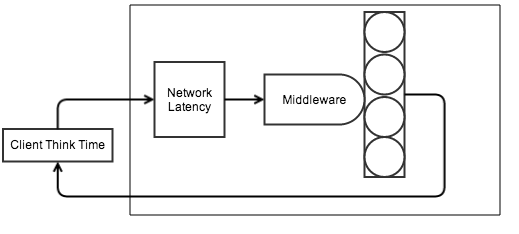
\includegraphics[width=0.8\linewidth]{firstmodel}
		\rule{35em}{0.5pt}
	\caption{Diagram over the first model applied to the system, a closed product form network.}
	\label{fig:firstmodel}
\end{figure}

	\subsection{Stations}
		\subsubsection{Network Latency}
		The network latency in this model includes actual real network latency but also includes the time it takes for the real middleware to create a new job and insert it into the worker-threadpool queue and also to send back a response to the client. This service time was measured to be on average 0.4 ms.

		\subsubsection{Middleware}
		This load independent service center has m servers where m represents the number of worker threads. The service time for the middleware in this first attempt model is 4.4 ms (measured from experiment using 10 worker threads).

	\subsection{Results}
	\begin{figure}[cht!]
		\centering
			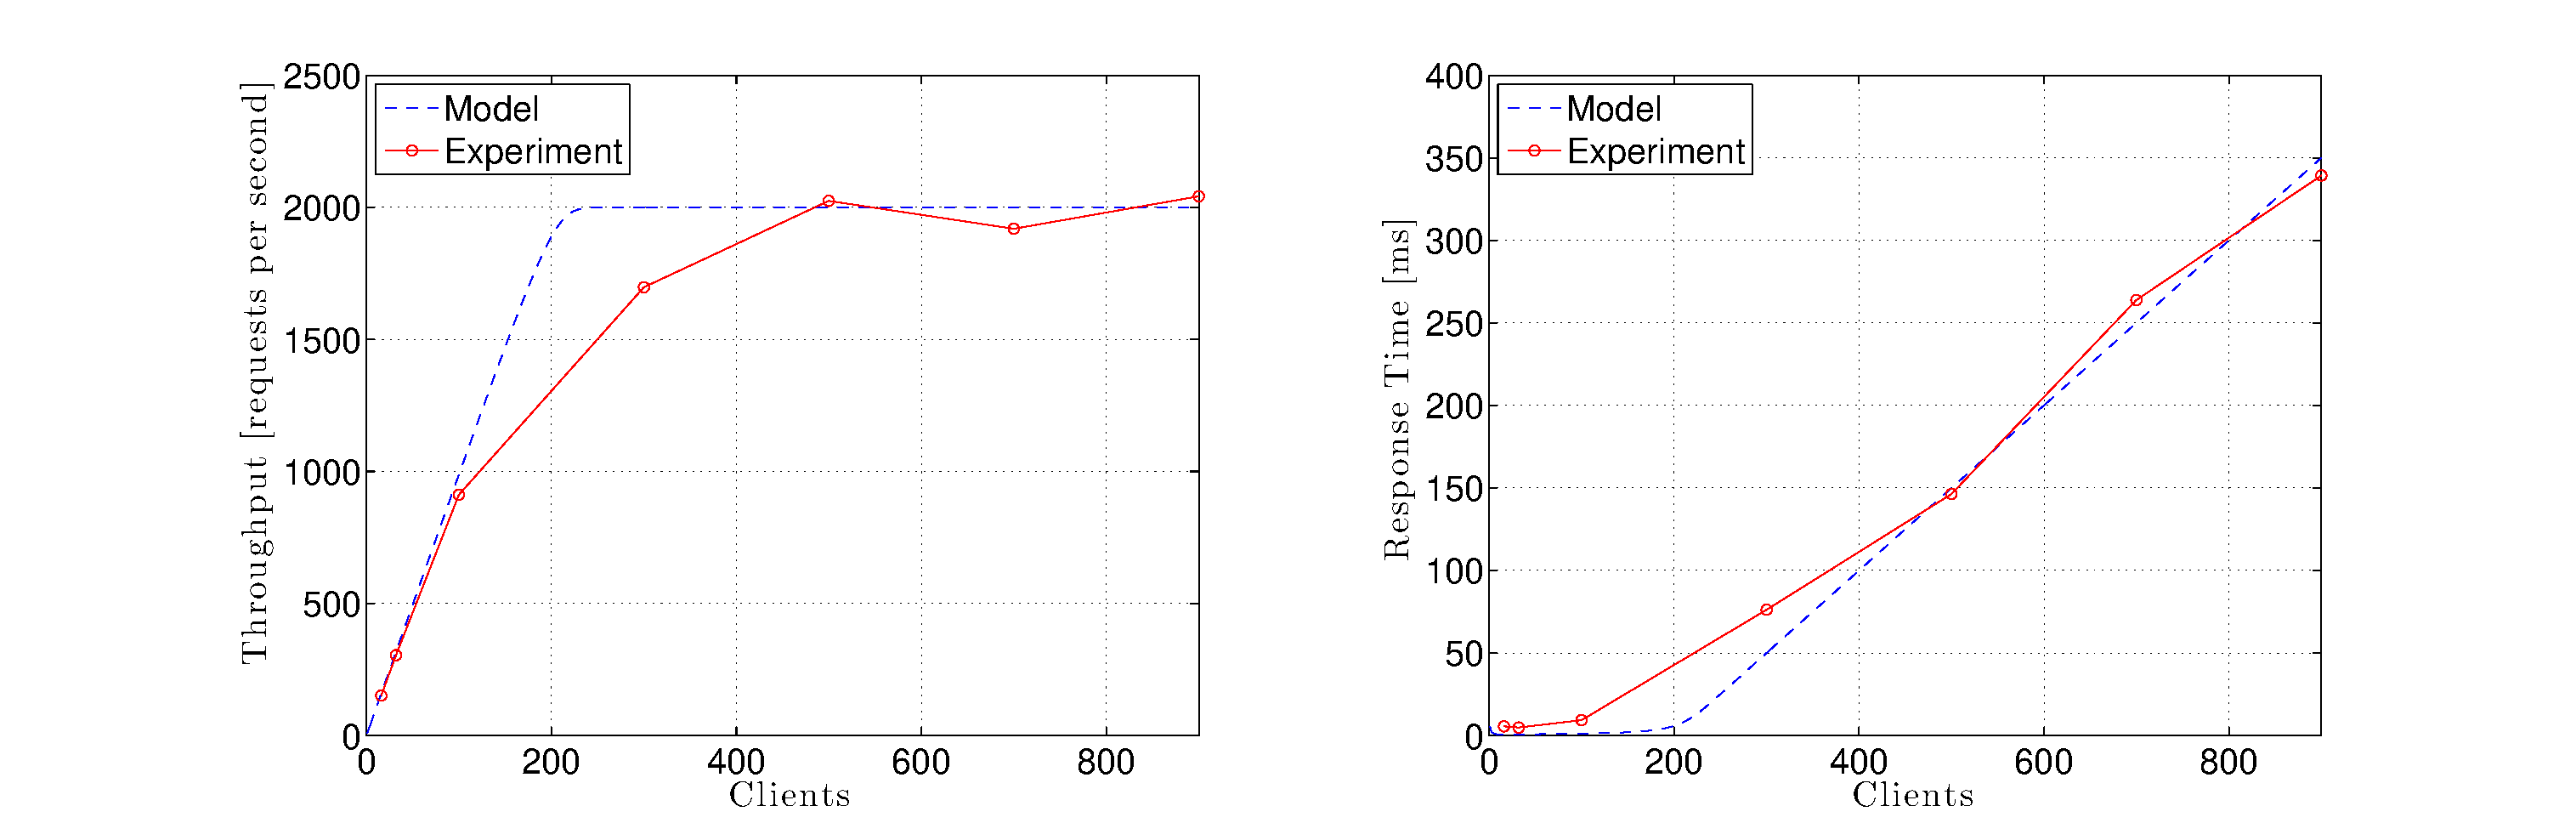
\includegraphics[width=1\linewidth,keepaspectratio]{firstRealAndModelRespAndThroughput}
		\caption{Diagram over the second model's response time and throughput compared with the experiment data of the system, using 10 middleware servers and think time of 100ms.}
		\label{fig:firstmodelResults}
	\end{figure}
	\FloatBarrier

	\subsection{Limitations and Analysis}
		The real system behaves sub-linear until it reaches saturation. The model behaves linearly. The sub-linearity depends on the increasing service time for the middleware when the number of concurrent requests increases. 
		The model introduced fairly work only when using 10 worker threads, highering the number of worker threads will make it inconsistent with the experiment. See Figure \ref{fig:firstmodelResultsFail} for an example where this model fails when using 80 working threads. The reason for this is that in this model the middleware is modeled as a load independent station while in reality the service time is dependent on the number of concurrent requests being processed. This is caused by contention in the database. To solve this problem, a new model is created with the persistence component modelled as a load dependent station.

		\begin{figure}[cht!]
			\centering
				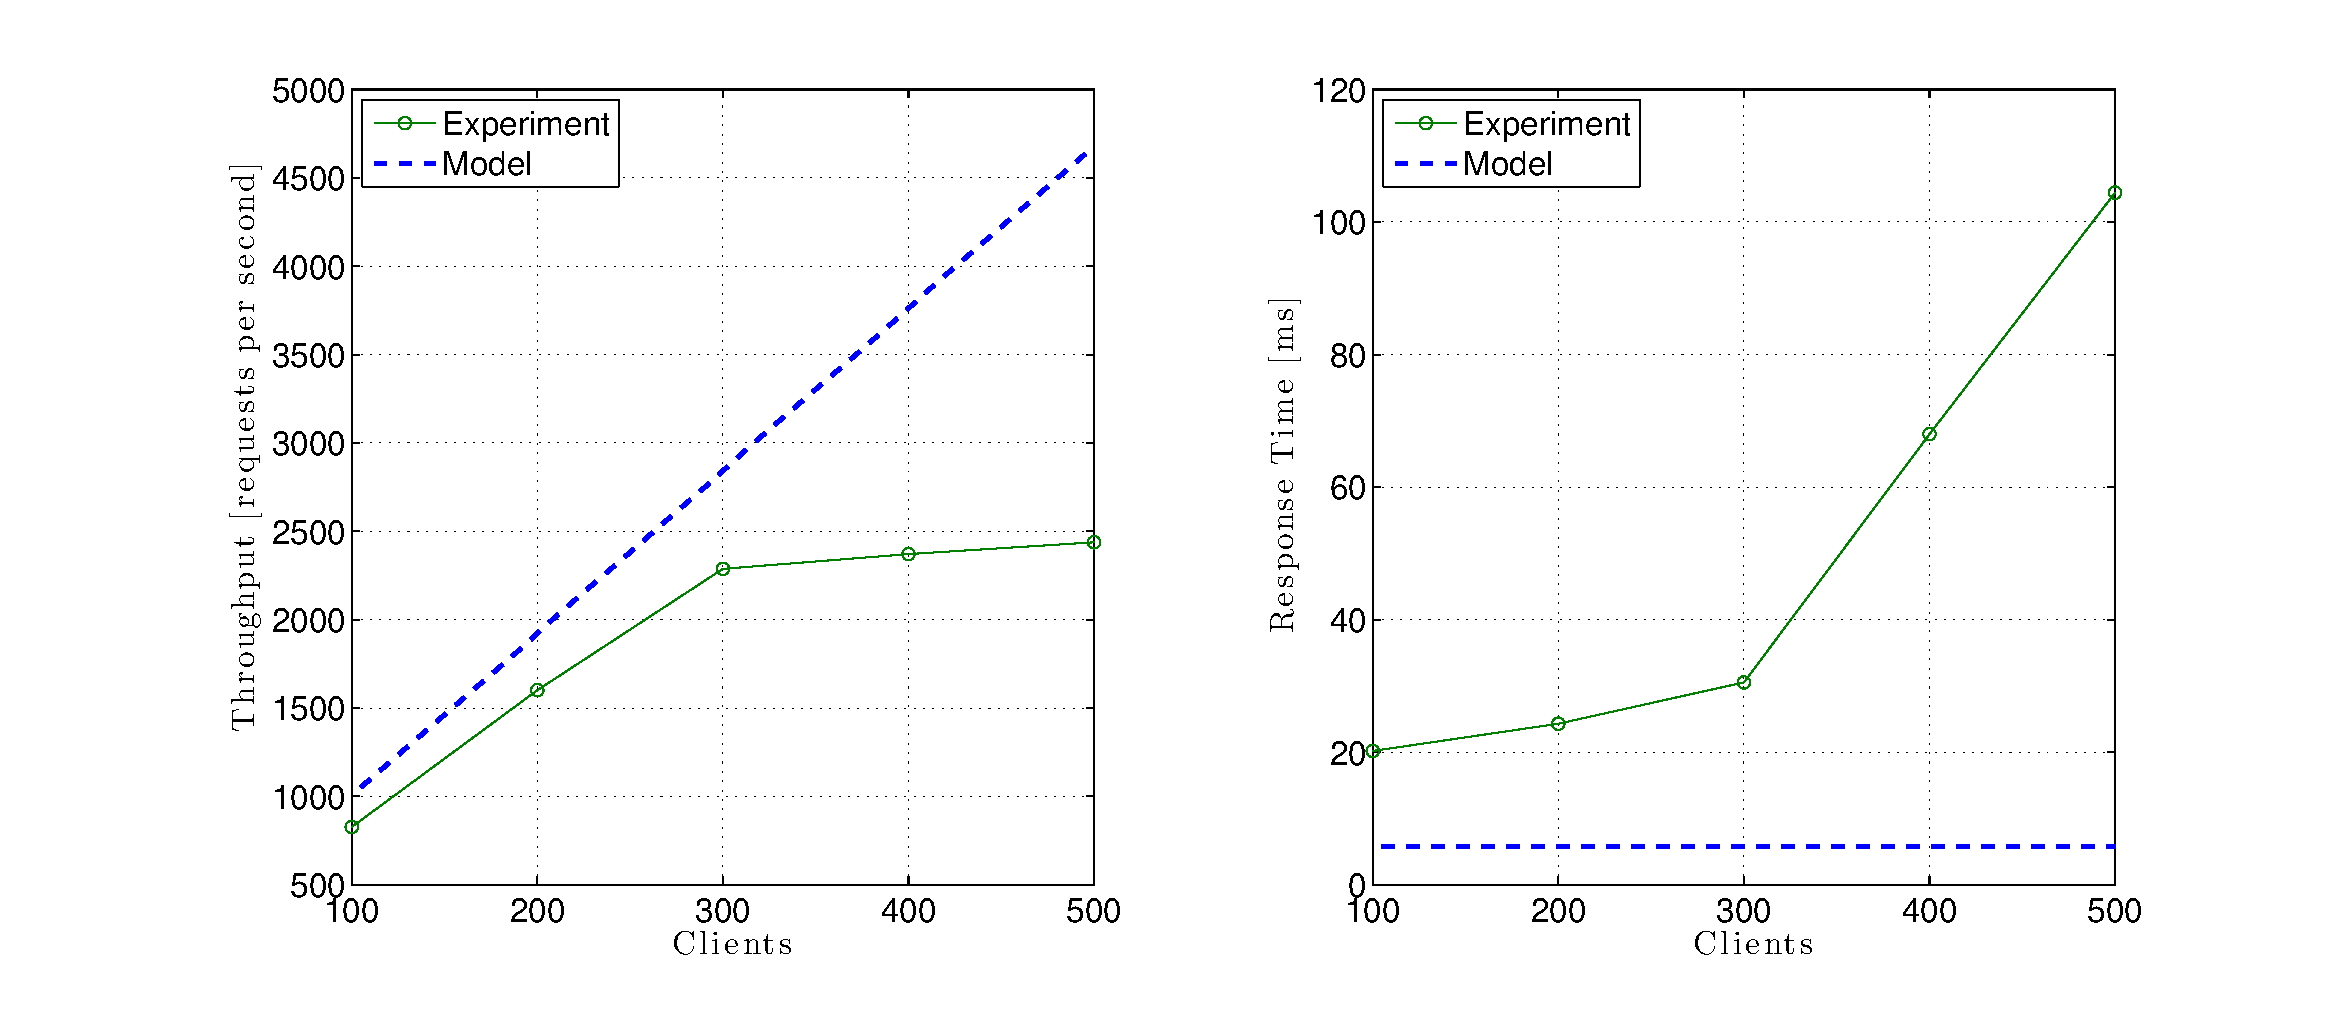
\includegraphics[width=1\linewidth,keepaspectratio]{firstRealAndModelFail}
			\caption{Diagram over the second model's response time and throughput compared with the experiment data of the system, using 80 middleware servers and think time of 100ms. The model fails to predict the actual performance of the system since in reality the middleware's service time is load dependent.}
			\label{fig:firstmodelResultsFail}
		\end{figure}
		\FloatBarrier


\section{Introducing Load Dependent Persistence}\label{sec:second-model}

	The second attempt involved increasing the resolution and more importantly introducing load dependency into the model. A diagram of the topology can be seen in Figure \ref{fig:second-model}.

	\FloatBarrier
	\begin{figure}[cht!]
		\centering
			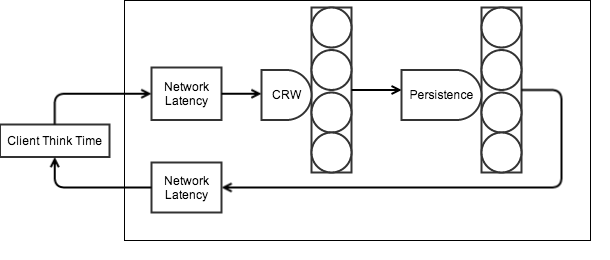
\includegraphics[width=0.8\linewidth]{secondmodel}
			\rule{35em}{0.5pt}
		\caption{Diagram over the second model applied to the system, a higher resolution model than the first attempt.}
		\label{fig:second-model}
	\end{figure}
	\FloatBarrier

\subsection{Stations}

	In this model the middleware station from the first attempt have been split into two parts: one for the client request worker component and one for the persistence component. The network latency have been split into two parts: one before and one after the client think time representing the time it takes to send to the middleware and one representing the time it takes to send a response.

	\subsubsection{Network Latency}
		This station have had it's service time halved but the number of visits have been doubled, so the total network latency is the same as the first model but is it more realistically inserted into the request flow. Modelled as a delay center.

	\subsubsection{CRW}
		The CRW is the part of the system which parses requests and build responses. This is modelled as a load independent station with service time 0.2 ms.

	\subsubsection{Persistence}
		This is the most crucial change in this new attempt. The service time for this is modelled to be load dependent on the number of jobs \textit{currently being processed}; it does not depend in queue length. The service times this is modell from can be seen in Figure \ref{fig:db-service-time}, and in a more explicit form (in milliseconds):
		\[ E[s] = 0.07941n^{1.353} + 2.859 ms\]

		where n is the number of jobs currently being processed.

		\begin{figure}[cht!]
			\centering
				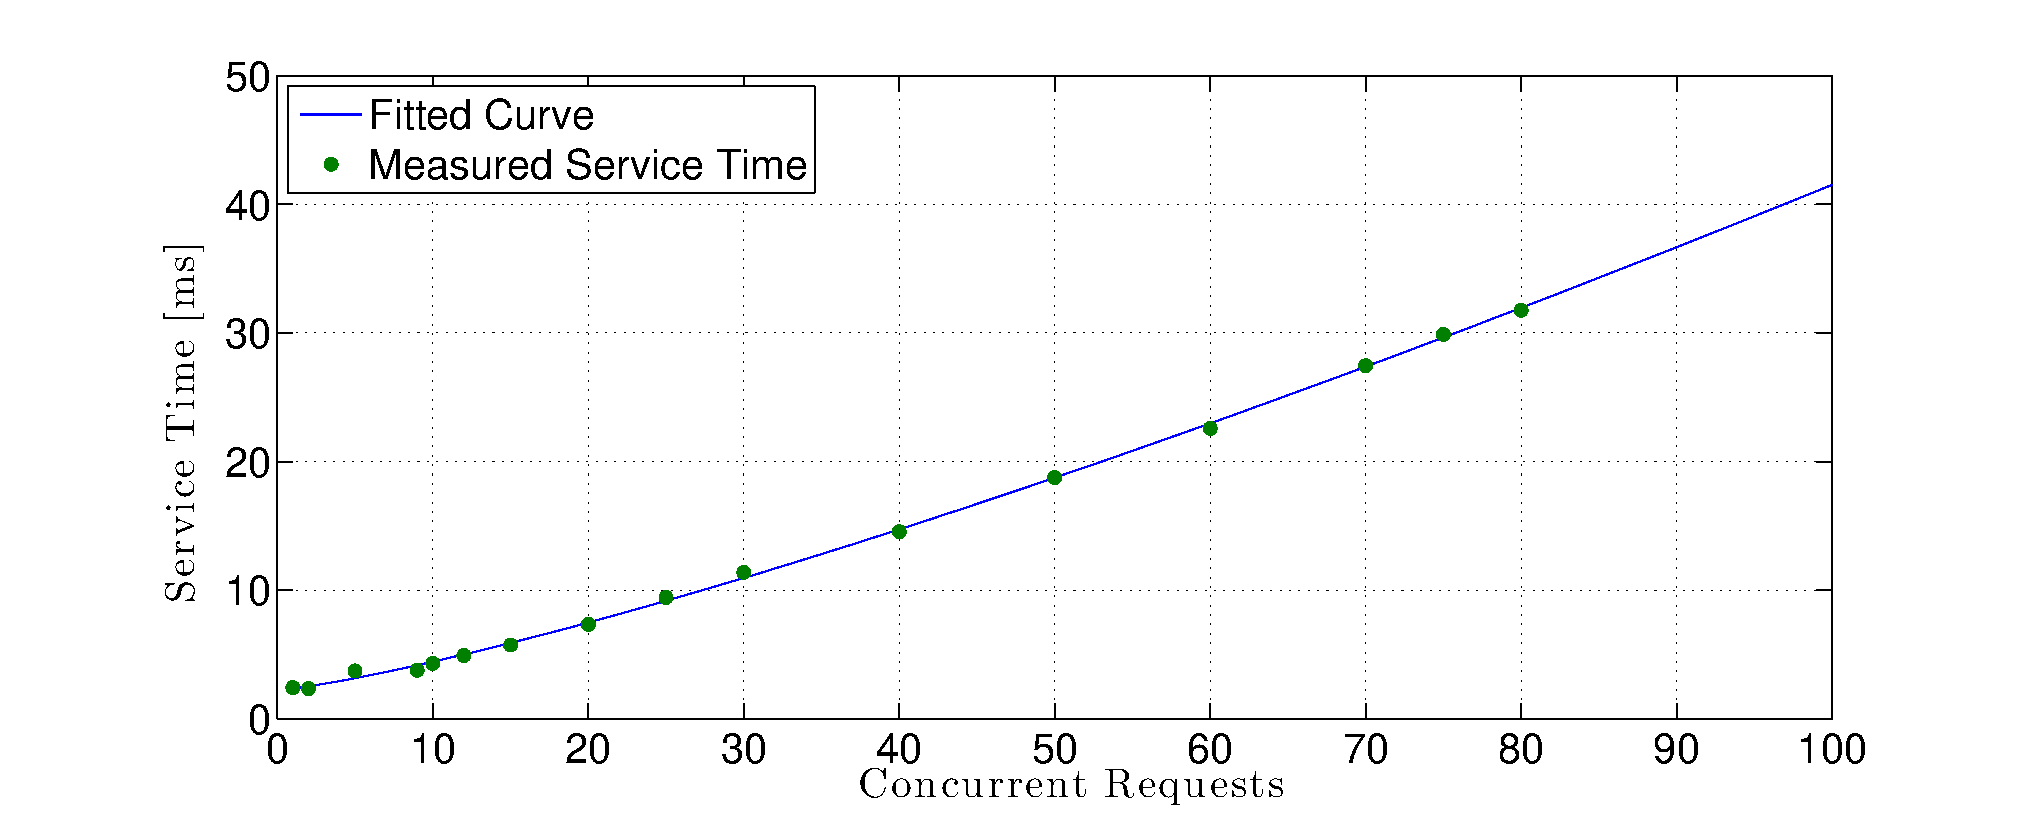
\includegraphics[width=\linewidth]{dbServiceTime}
				\rule{35em}{0.5pt}
			\caption{The service time for the database component as a function of the number of concurrent requests being processed.}
			\label{fig:db-service-time}
		\end{figure}
		\FloatBarrier
	
\subsection{Results}
	This model predicts the performance of the system much better than the first model did, this is thanks to the load dependency in the persistence component.
	\FloatBarrier
	\begin{figure}[cht!]
		\centering
			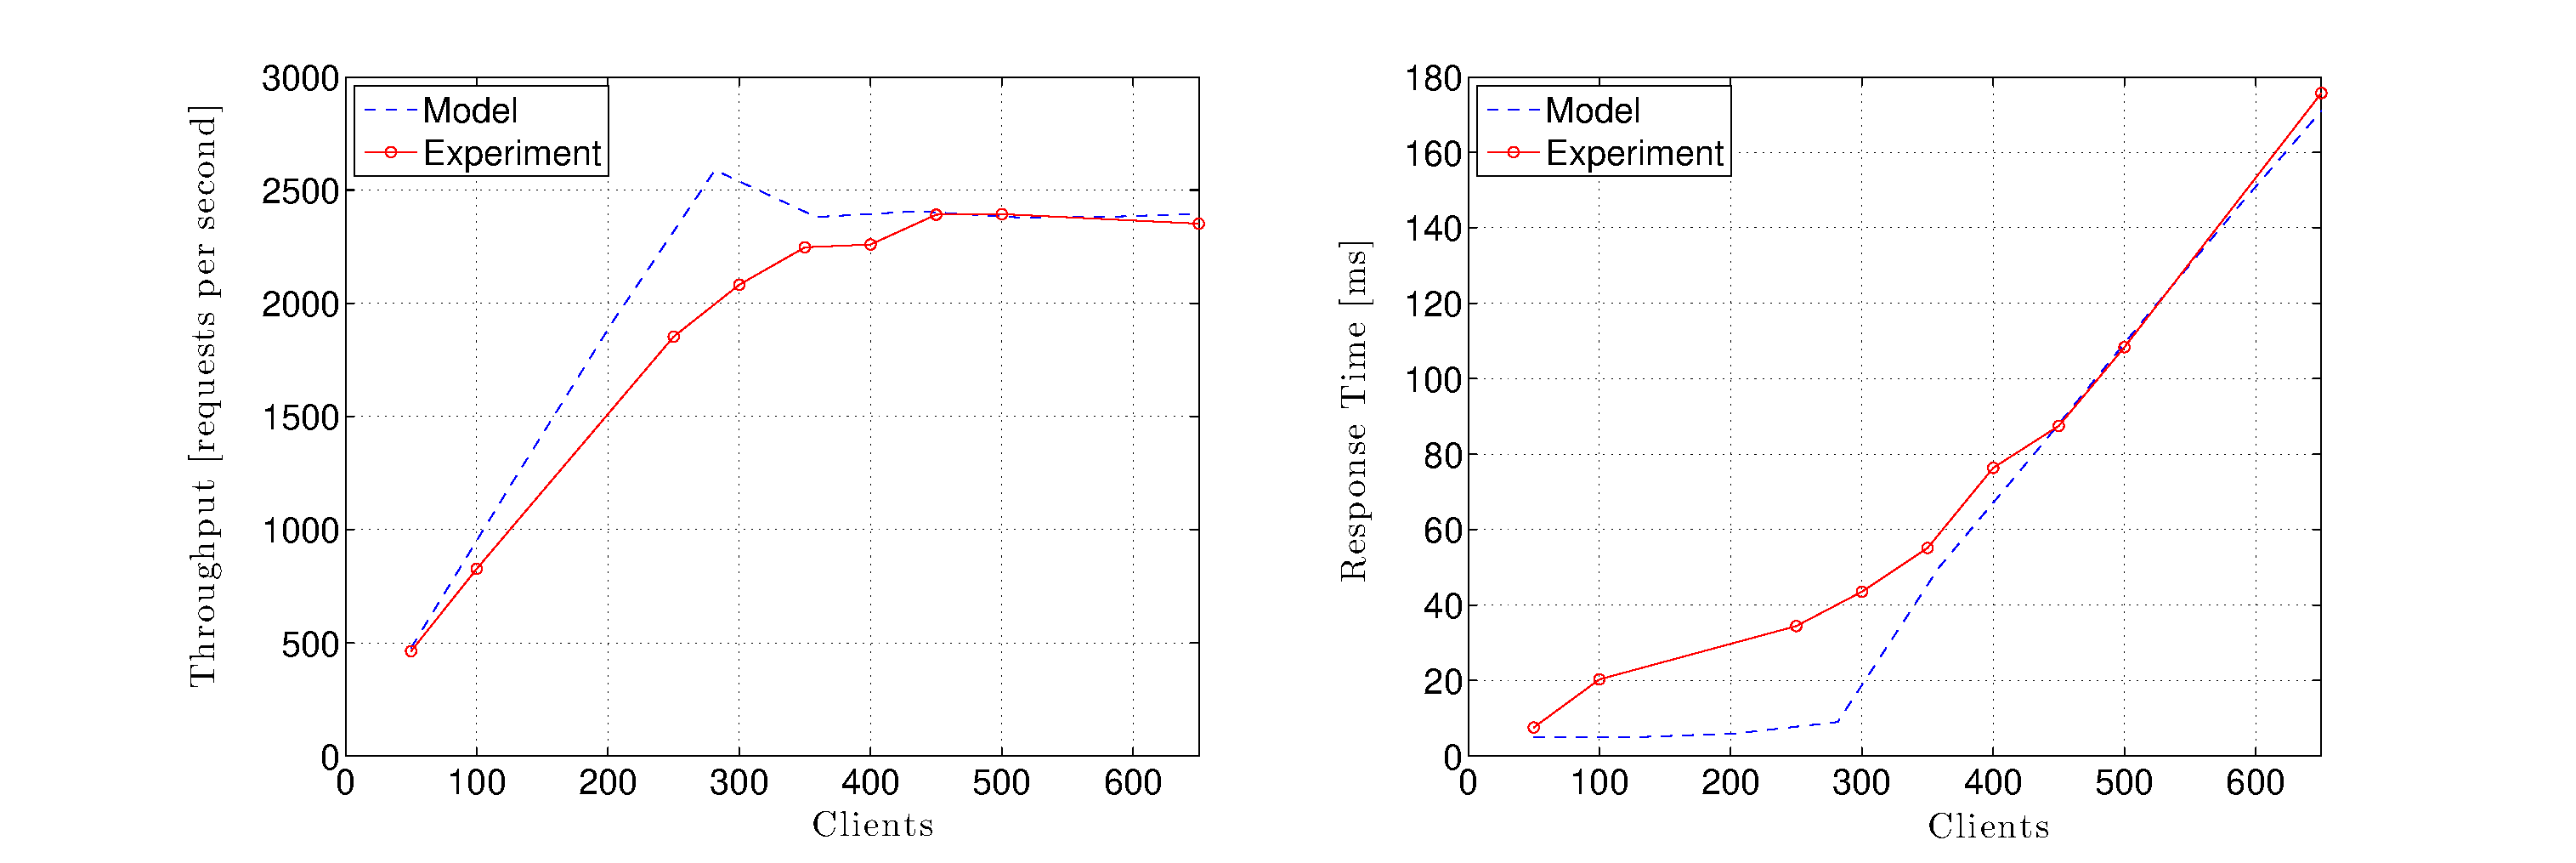
\includegraphics[width=1\linewidth,keepaspectratio]{secondRealAndModel}
		\caption{Diagram over the second model's response time and throughput compared with the experiment data of the system, using 80 CRW servers and 80 Persistence servers and think time of 100ms. This model calculates better results than the first attempt, since this model takes congestion in the database into account.}
		\label{fig:secondmodelResults}
	\end{figure}
	\FloatBarrier
	\begin{figure}[cht!]
		\centering
			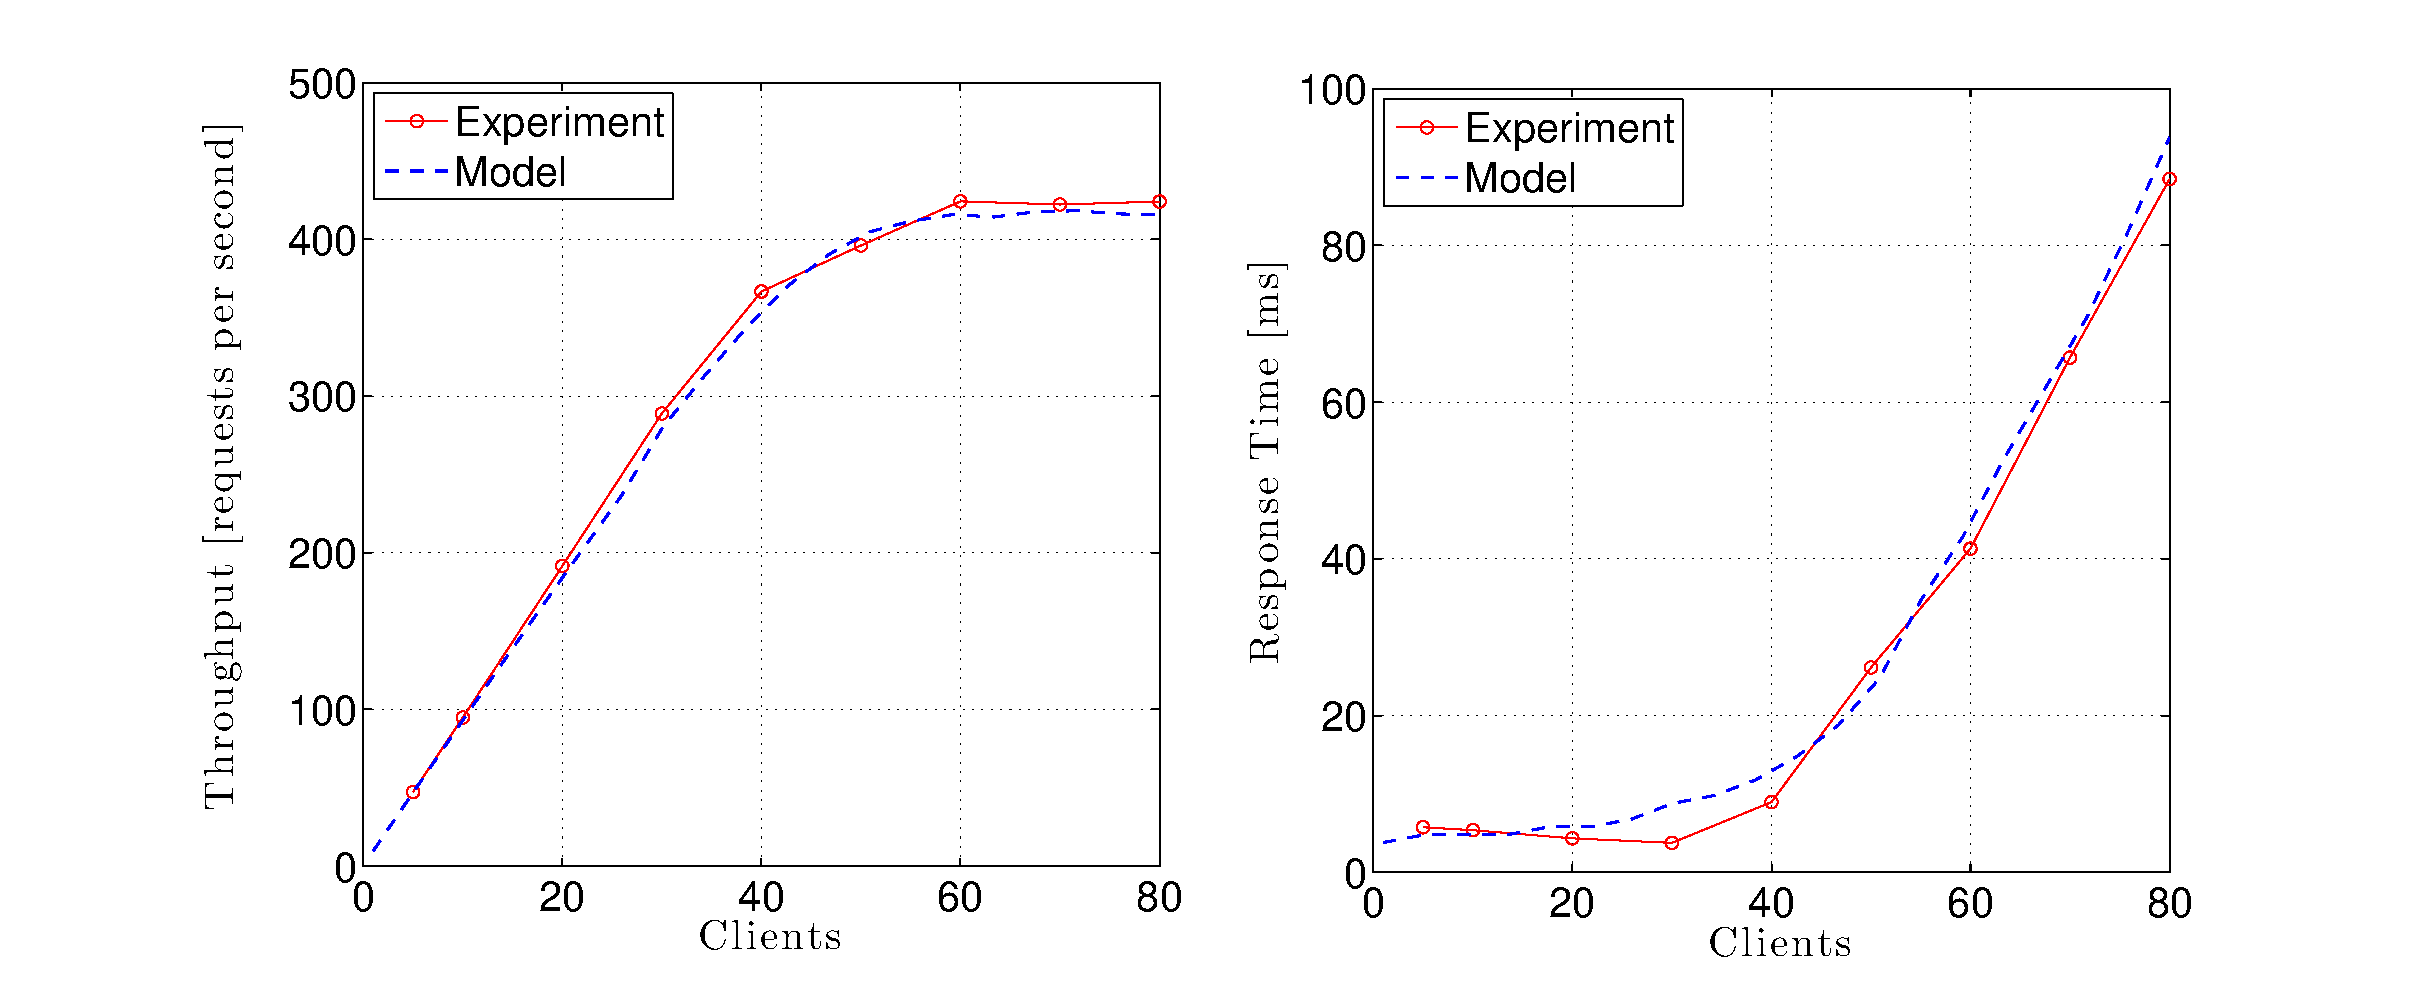
\includegraphics[width=1\linewidth,keepaspectratio]{secondRealAndModel1Thread}
		\caption{Diagram over the second model's response time and throughput compared with the experiment data of the system, using 1 CRW servers and 1 Persistence servers and think time of 100ms. Good fit with the experiment data.}
		\label{fig:secondmodelResults-1-th}
	\end{figure}
	\FloatBarrier

	\subsection{Limitations and Analysis}
	The model corresponds generally well with the true performance with regards to the asymptotes of response time and throughput. But before the system reaches saturation the model does not predict well when using a high number of worker heads, see Figure \ref{fig:secondmodelResults-error}. 

	\FloatBarrier
	\begin{figure}[cht!]
		\centering
			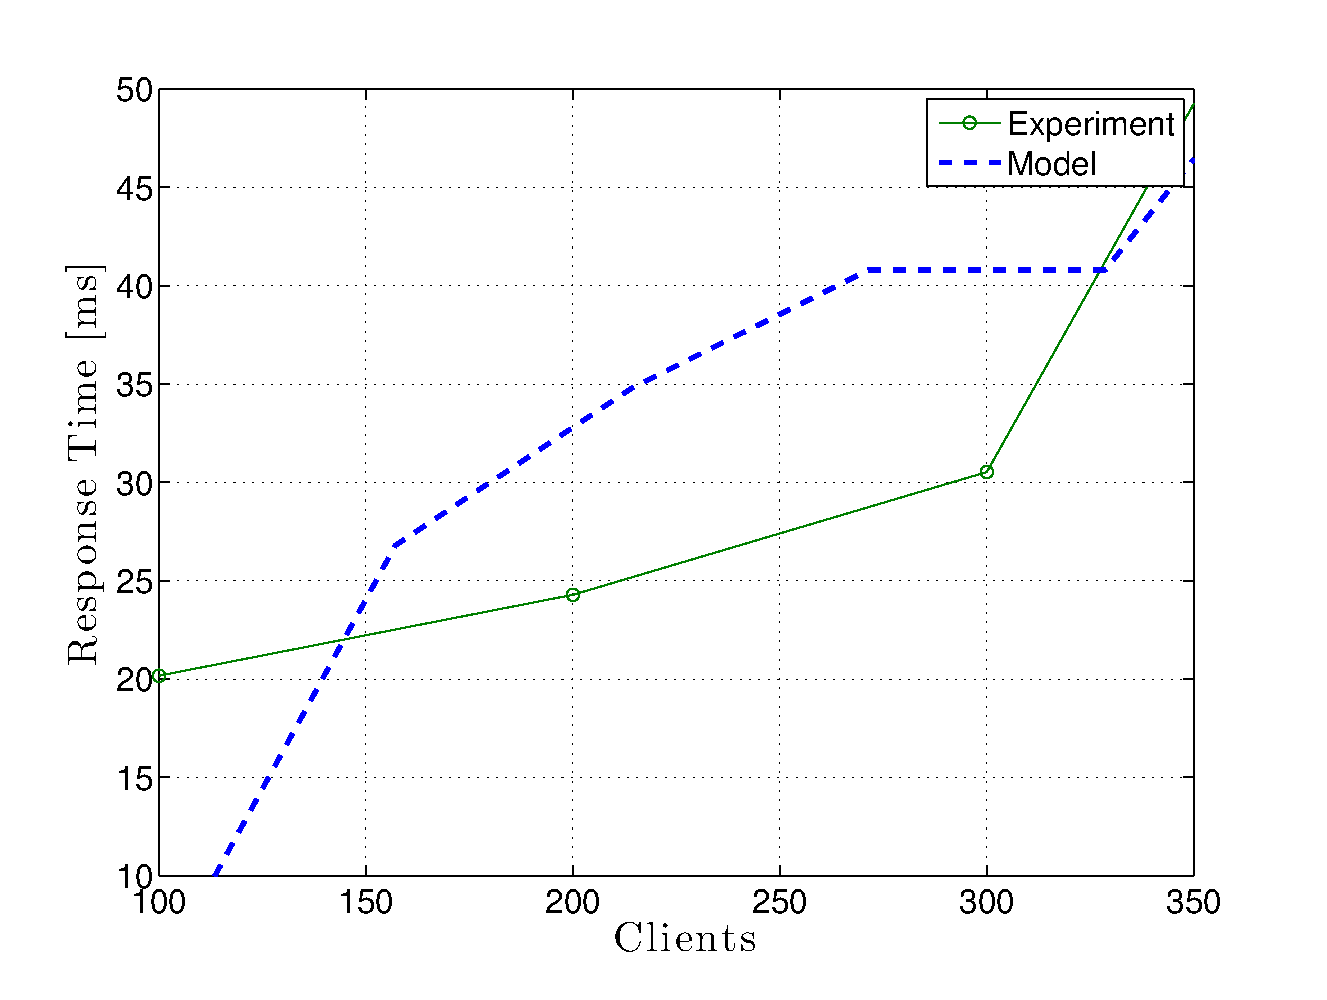
\includegraphics[width=1\linewidth,keepaspectratio]{secondRealAndModelError}
		\caption{Misprediction of the second model before the system reaches saturation.}
		\label{fig:secondmodelResults-error}
	\end{figure}
	\FloatBarrier

	Another thing one can notice from the model is the peak of throughput in Figure \ref{fig:second-model} just before the system reaches saturation. This peek seems to indicate that using 80 database connections simultaneously is not the optimal and suggests that the optimal number is rather lower. Looking and the expected queue lengths for the data-points showed that the number of expected clients in the persistence component for this point was around 30. So, a new test was run with 30 data-base connections, see Figure \ref{fig:secondRealAndModel30th}. 

	\FloatBarrier
	\begin{figure}[cht!]
		\centering
			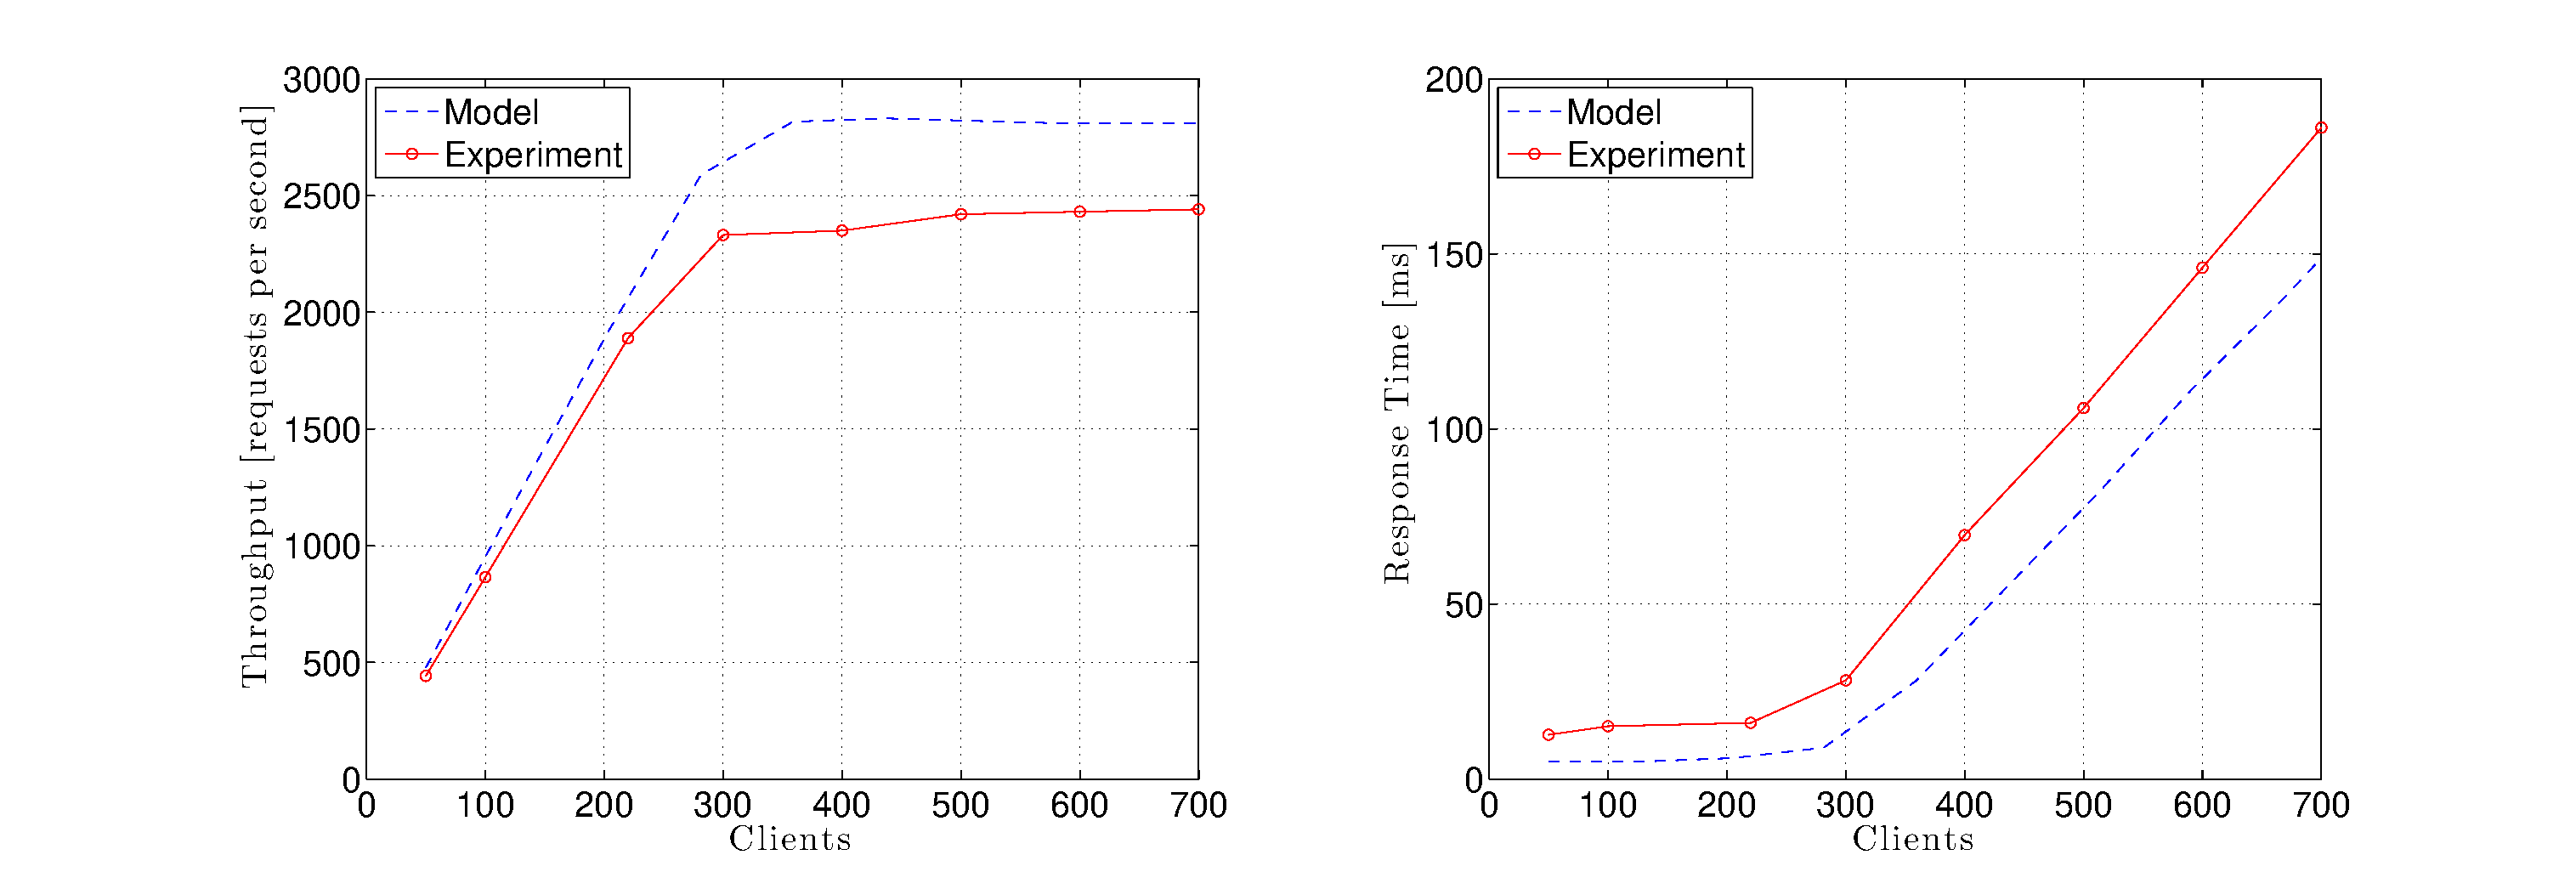
\includegraphics[width=1\linewidth,keepaspectratio]{secondRealAndModel30th}
		\caption{Misprediction of the second model when using 30 worker threads. This is attributed to overfitting of the service time model.}
		\label{fig:secondRealAndModel30th}
	\end{figure}
	\FloatBarrier

	This large error suggests that the model for the service time for the persistence component has been over-fitted to the measured data. New measurements were made with a special focus on the 1-10 concurrent requests where one-incremental tests were made. After this two linear models were fitted to the data points, one for the lower span and one for the upper span. This was made with an heuristic approach, no real theory supported this approach, but the fitted model seemed to fit well with the measured points. The fitted curves can be seen in Figure \ref{fig:newServiceTimeDb} and the model is more explicitly:
		\[ E[s](s) = \max\left(0.2515n+1.872, 0.4271n -0.3985\right) \]
	where $n$ is the number of jobs being processed simultaneously.


	\FloatBarrier
	\begin{figure}[cht!]
		\centering
			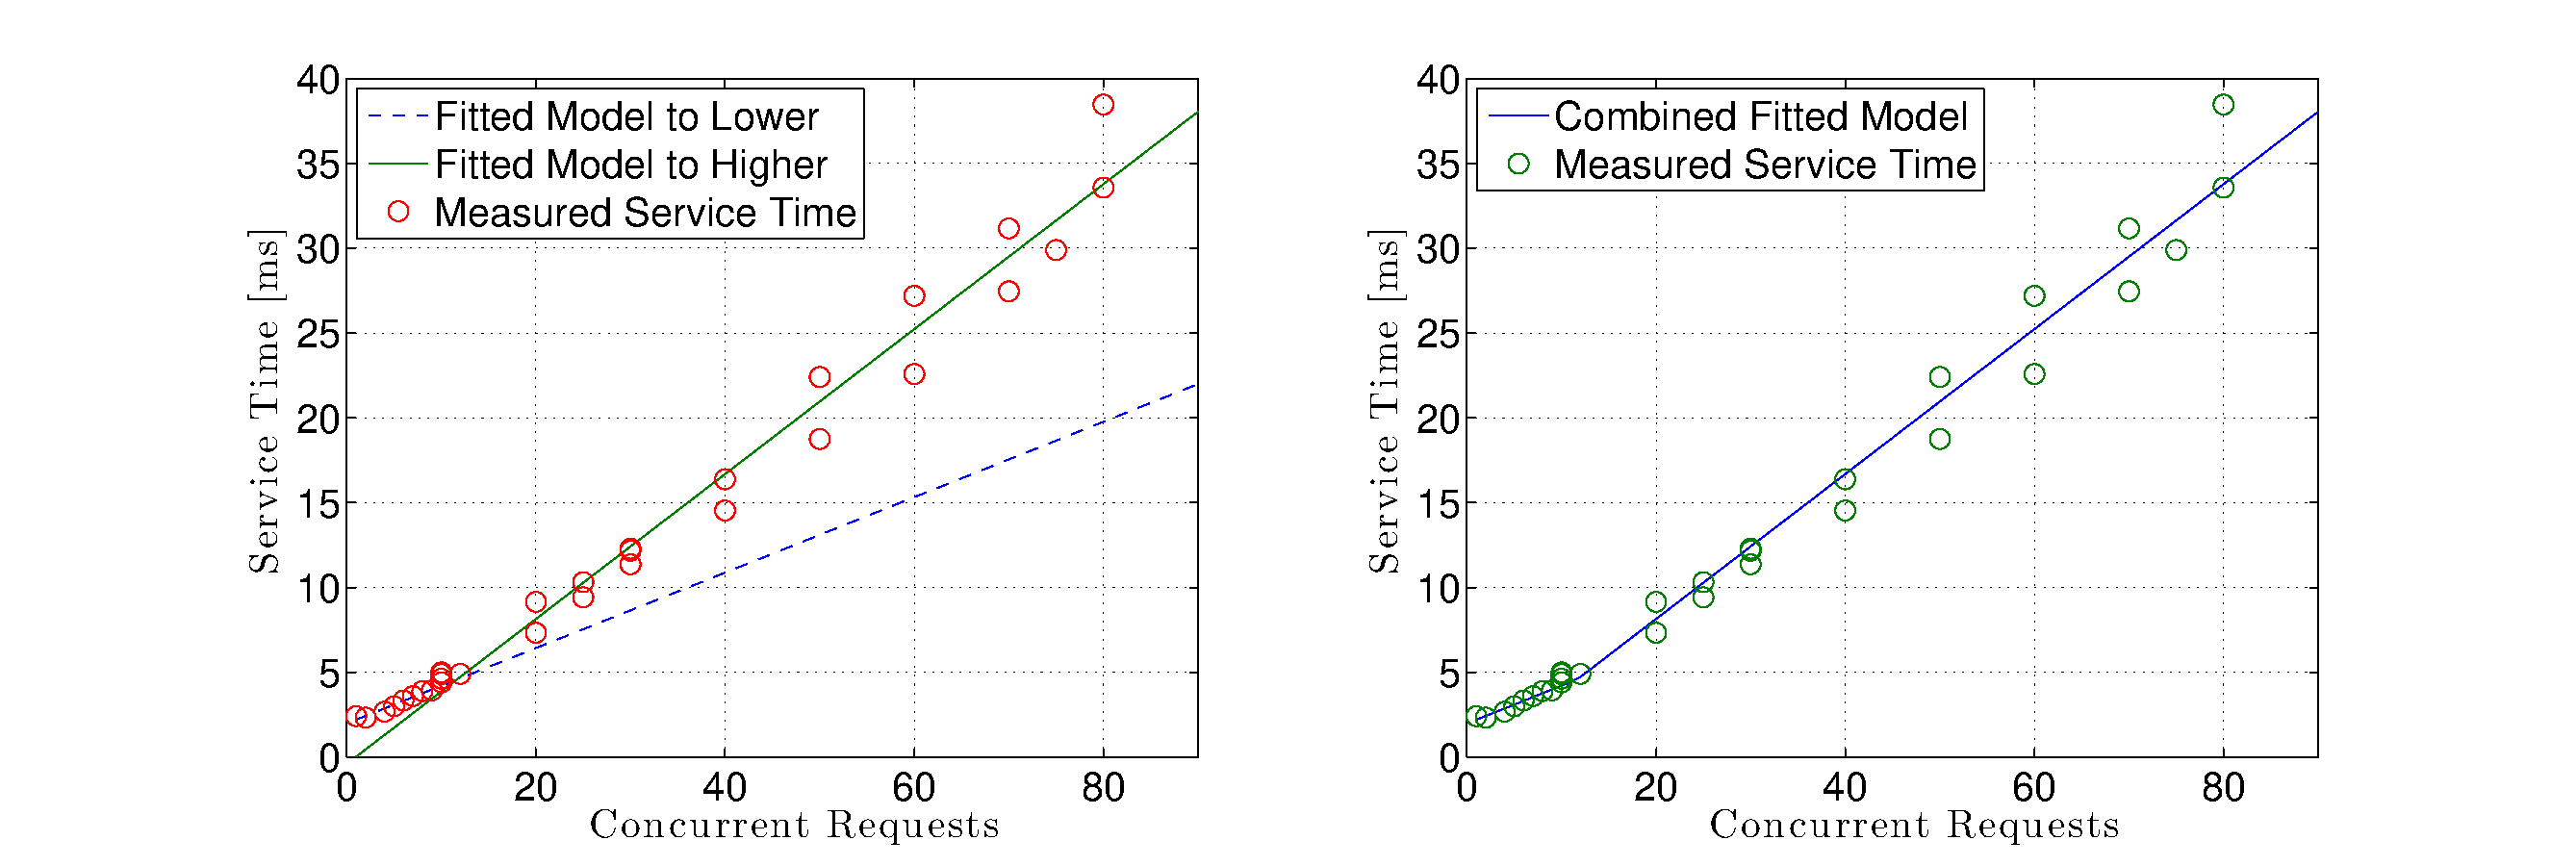
\includegraphics[width=1\linewidth,keepaspectratio]{newServiceTimeDb}
		\caption{The new model for the persistence component service times.}
		\label{fig:newServiceTimeDb}
	\end{figure}
	\FloatBarrier

\section{Final Model}
The final model has the same topology as the second model but with the revised model for the service times for the persistence station.

	\subsection{Results}
	 
	\FloatBarrier

	\begin{figure}[cht!]
		\centering
			\includegraphics[width=1\linewidth,keepaspectratio]{thirdRealAndModel10Th}
		\caption{The prediction of the model versus the experiment data with the new model for the persistence service times when using 10 worker threads and $Z = 0.1$.}
		\label{fig:thirdRealAndModel10Th}
	\end{figure}

	\begin{figure}[cht!]
		\centering
			\includegraphics[width=1\linewidth,keepaspectratio]{thirdRealAndModel30Th}
		\caption{The prediction of the model versus the experiment data with the new model for the persistence service times when using 30 worker threads and $Z = 0.1$.}
		\label{fig:thirdRealAndModel30Th}
	\end{figure}

	\begin{figure}[cht!]
		\centering
			\includegraphics[width=1\linewidth,keepaspectratio]{thirdRealAndModel80Th}
		\caption{The prediction of the model versus the experiment data with the new model for the persistence service times when using 80 worker threads and $Z = 0.1$.}
		\label{fig:thirdRealAndModel80Th}
	\end{figure}
	\FloatBarrier


	\subsection{Limitations and Analysis}
	This model predicts more accurately than the second model and this is due to the new model for the service times for the persistence component. Although it is more consistent with the experiment there appears to be a tendency for the real system to behave more and more sub-linearly when increasing the number of worker threads and database-connections. The reason for this must lie outside the persistence component and perhaps the culprit lies in the socket I/O component, since it is the only component which has not been analyzed further since it was assumed to be load independent. Perhaps there is contention when having so many simultaneously requesting going back and forth, though there is no more time to further analyze the system.


\section{Scaling}
	One question one can ask is how does the model differentiate between scaling out and scaling up (essentially more threads vs more middleware). The answer is that since the bottle-neck is neither the working threads nor the middleware it makes no difference if the system is using 10 threads in each 8 middlewares or if it is using 80 threads in one middleware since the limiting factor is the database, given that increasing the number of threads to 80 does make the middleware the bottleneck (which is not the case in this system, but may hold in another system). This is  supported by experiments, see Figure \ref{fig:1mw80th-vs-8mw10th}. So to model a setup which corresponds to using 3 middleware with 10 threads each, set the number of CRW and Persistence servers each to 30.

	\FloatBarrier
	\begin{figure}[cht!]
		\centering
			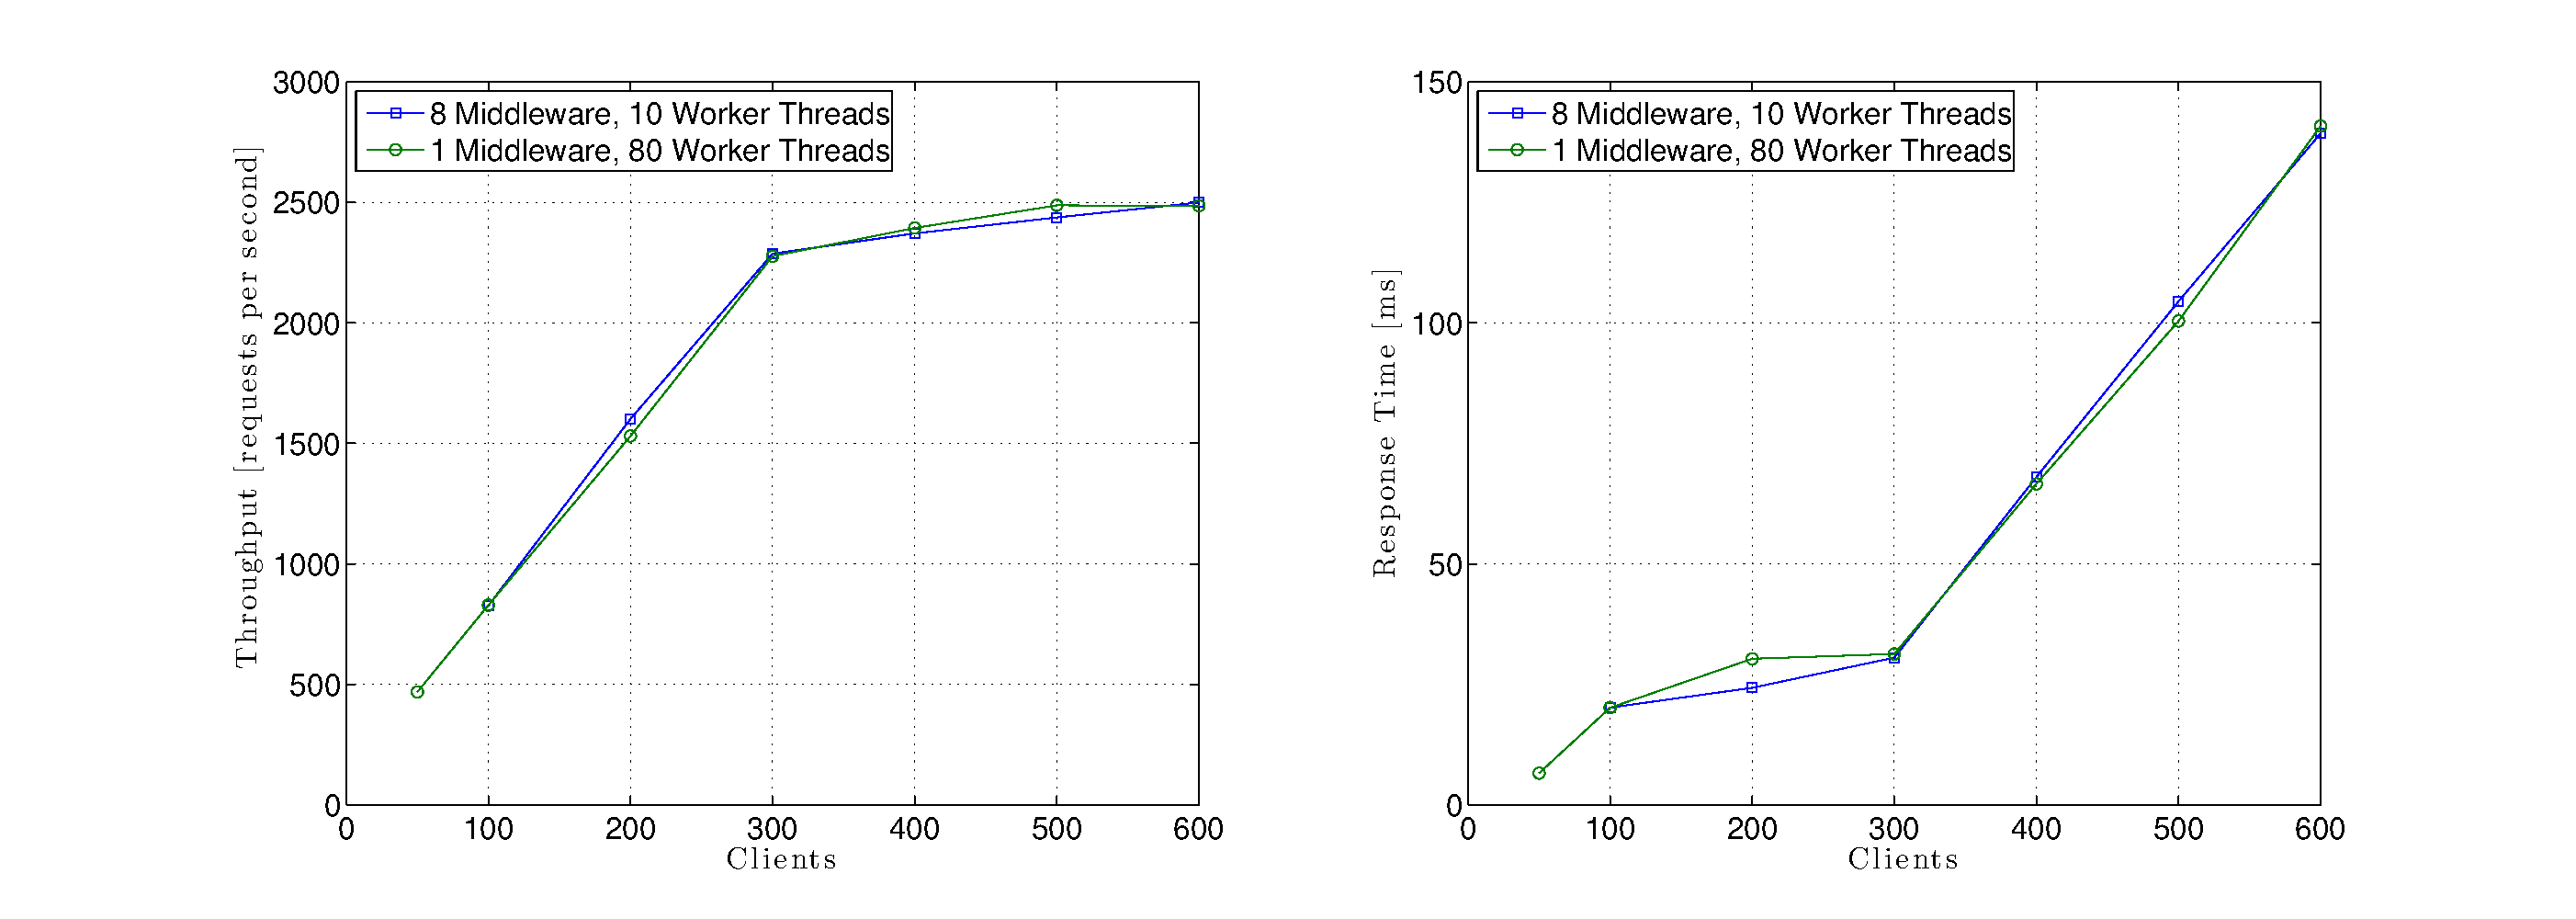
\includegraphics[width=1\linewidth,keepaspectratio]{1mw80th-vs-8mw10th}
		\caption{The throughput and response time of the system while using 1 middleware and 80 worker threads (and 80 db-connections) versus using 8 middleware and 10 workers threads (and 10 db-connections) per middleware.}
		\label{fig:1mw80th-vs-8mw10th}
	\end{figure}
	\FloatBarrier


\section{Conclusion}
	The final model is a closed product form network with the topology showed in Figure \ref{fig:second-model} with these parameters:
	\FloatBarrier
	\begin{table}[cht!]
		\centering
		\begin{tabular}{|l|l|l|l|}
			\hline
			\textbf{Component} 		& \textbf{Type} 	& \textbf{Service Time (ms)} 	& \textbf{Visists} \\ \hline
			Network Latency 		& Delay Center 		& 0.2 						& 2 \\ \hline
			Client Request Worker 	& Load-Independent 	& 0.2 						& 1 \\ \hline
			Persistence 			& Load-Dependent 	& $\max\left(0.2515n+1.872, 0.4271n -0.3985\right)$ 					& 1 \\ \hline
		\end{tabular}
	\end{table}		
	\FloatBarrier

	The model predicts the system performance well, although when more worker threads and database-connections are used the real system behaves more sub-linearly than the model (which exhibits some sub-linearity as well). The conclusion is that for further development of the model measurements of the service time for the socket I/O components should be made. A suggested approach would be to split the Network Latency-component to one load independent and one Socket I/O-component which would represent the non-blocking socket logic in the middleware.

\section{Things Learned}
	This milestone provided much more insight and confidence in the system's performance and the effects of the parameters than the first milestone. It is also very important to have a stable testing setup. If I would have redone this milestone i would have made sure to never destroy and create new servers in the cloud for different tests\footnote{Tests were re-run to take advantage from the better measurement implementations, the system itself has not been changed at all} as new servers are not necessarily placed in the same host so the available computing power varies.\\

	The system behaves sub-linearly when the number of effective worker threads is increased which is due to the service time increases when many concurrent requests are being processed simultaneously.

\section{General Limitations}

	\subsection{Service Time Distributions}
		The models assume exponentially distributed service times, but the measurements show that this is not the case and it is also in it self unrealistic since the mode of the exponential distribution is 0, while in fact a service time of 0 never happens. A fitted probability density curve of a exponential distribution to the service time of the persistence component service times can be seen in Figure \ref{fig:serviceTimeDbHistogram10Threads} together with a PDF for a log normal distribution. It appears that the service time for the persistence component is log normally distributed and not exponential.

		\FloatBarrier
		\begin{figure}[cht!]
			\centering
				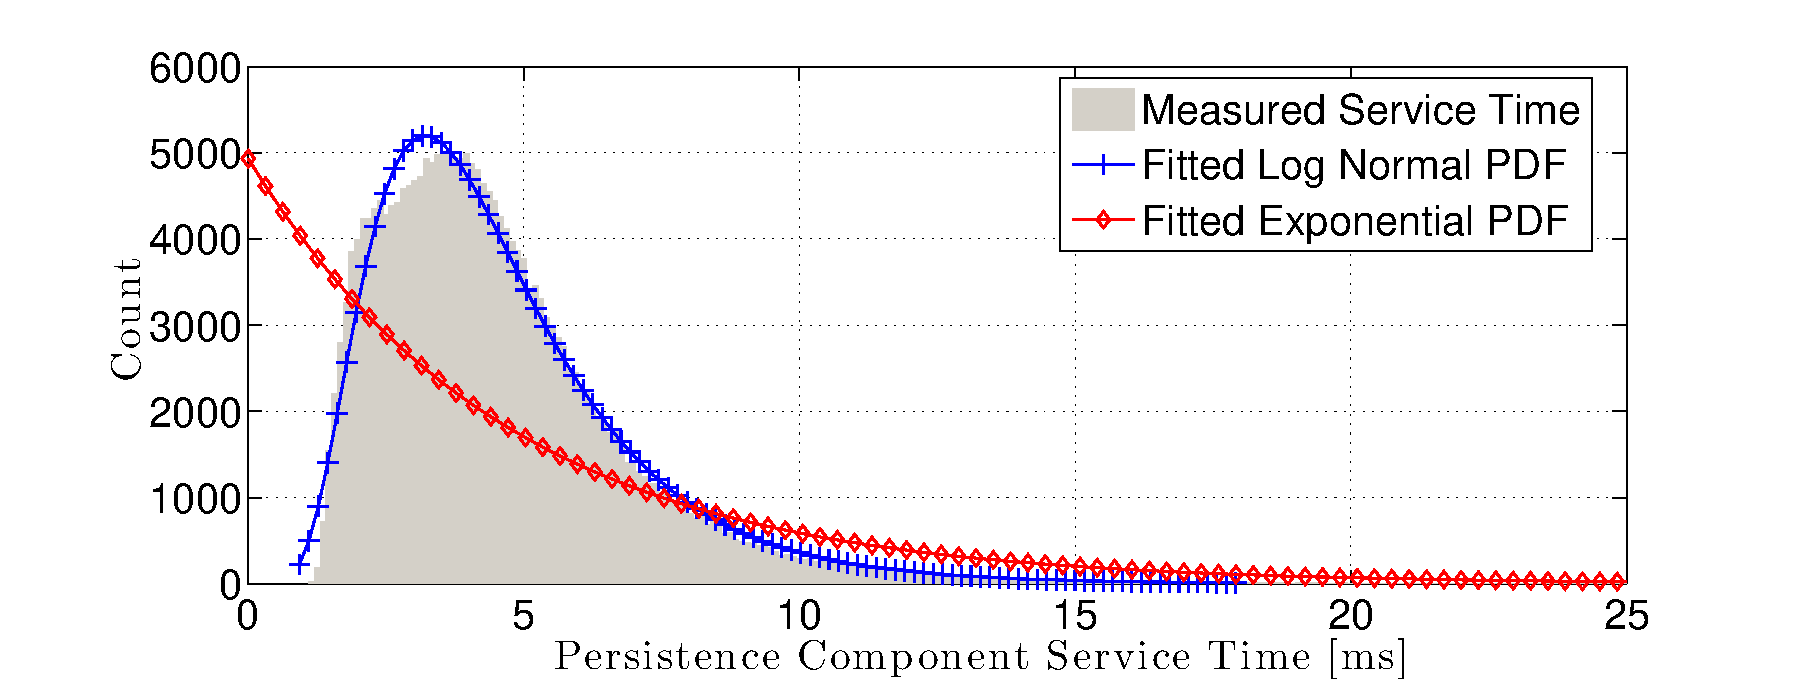
\includegraphics[width=1\linewidth,keepaspectratio]{serviceTimeDbHistogram10Threads}
			\caption{The distribution of the persistence component service time along with a fitted exponential distribution probability density curve (PDF) and a log normal PDF.}
			\label{fig:serviceTimeDbHistogram10Threads}
		\end{figure}
		\FloatBarrier

		\subsubsection{Implication}
			According to Rai Jain, 1991, p. 620-621, the distribution of the services times mostly affect the predicted device utilization and the error in the prediction for the response times and queue length is much less compared. According to Suri (1983, Robustness of Queueing Network Formulas) the difference is not significant.

	\subsection{Software Limitations vs. Model}
		The software, more specifically PostgreSQL, has some limitation which the model does not take into account. One of these limitations is the number of concurrent database connections. While in reality the PostgreSQL has a limit on the number of open connections and the model could scale this into infinity. So the model holds with the parameters within certain intervals: the Persistence component can for example be modelled as a $M/M/m$ where $m \in [1,100]$ ($\in \mathbb{N}$). The \texttt{ThreadPoolExecutor} used in the middleware for thread-pooling the worker threads could also be modelled with an arbitrarily big pool size. The CRW component is modelled as a load independent station, so the service times for the modelled CRW may not hold as the service times may go up when using a large number of concurrent worker threads. No service time measurements for CRW service times have been done for $m > 80$ though, so no implicative statement can be made in this regard.

	\subsection{Hardware Coupling}
		Because of the tests and measurements are done on the same hardware throughout the milestone, this model is coupled to the specific hardware used. One thing that would be very benefitial would be to measure how the performance changes with respect to the amount of RAM and the performance of the CPU. If it would be possible to fit a model to these parameters and given that there is a model for the service times for the system the "perfect match" could be calculated.
\end{document} 
